% Figure: Clift 5-stage lifting pipeline
\begin{figure}[t]
\centering
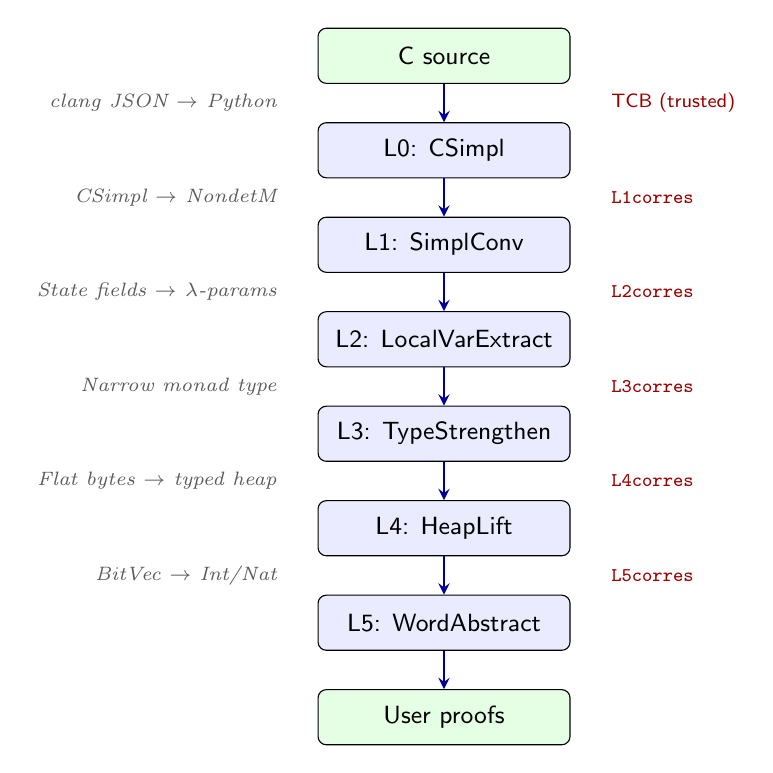
\begin{tikzpicture}[
  stage/.style={draw, rounded corners=3pt, fill=blue!8, minimum width=3.2cm,
                minimum height=0.7cm, font=\small\sffamily},
  arrow/.style={->, >=stealth, thick, color=blue!60!black},
  label/.style={font=\scriptsize\itshape, text=gray!70!black},
  corres/.style={font=\scriptsize\sffamily, text=red!60!black},
]
  % Stages
  \node[stage, fill=green!10] (c) at (0, 0) {C source};
  \node[stage] (l0) at (0, -1.2) {L0: CSimpl};
  \node[stage] (l1) at (0, -2.4) {L1: SimplConv};
  \node[stage] (l2) at (0, -3.6) {L2: LocalVarExtract};
  \node[stage] (l3) at (0, -4.8) {L3: TypeStrengthen};
  \node[stage] (l4) at (0, -6.0) {L4: HeapLift};
  \node[stage] (l5) at (0, -7.2) {L5: WordAbstract};
  \node[stage, fill=green!10] (proof) at (0, -8.4) {User proofs};

  % Arrows between stages
  \draw[arrow] (c) -- (l0);
  \draw[arrow] (l0) -- (l1);
  \draw[arrow] (l1) -- (l2);
  \draw[arrow] (l2) -- (l3);
  \draw[arrow] (l3) -- (l4);
  \draw[arrow] (l4) -- (l5);
  \draw[arrow] (l5) -- (proof);

  % Transform labels (left)
  \node[label, anchor=east] at (-2.0, -0.6) {clang JSON $\to$ Python};
  \node[label, anchor=east] at (-2.0, -1.8) {CSimpl $\to$ NondetM};
  \node[label, anchor=east] at (-2.0, -3.0) {State fields $\to$ $\lambda$-params};
  \node[label, anchor=east] at (-2.0, -4.2) {Narrow monad type};
  \node[label, anchor=east] at (-2.0, -5.4) {Flat bytes $\to$ typed heap};
  \node[label, anchor=east] at (-2.0, -6.6) {BitVec $\to$ Int/Nat};

  % Corres labels (right)
  \node[corres, anchor=west] at (2.0, -0.6) {TCB (trusted)};
  \node[corres, anchor=west] at (2.0, -1.8) {\texttt{L1corres}};
  \node[corres, anchor=west] at (2.0, -3.0) {\texttt{L2corres}};
  \node[corres, anchor=west] at (2.0, -4.2) {\texttt{L3corres}};
  \node[corres, anchor=west] at (2.0, -5.4) {\texttt{L4corres}};
  \node[corres, anchor=west] at (2.0, -6.6) {\texttt{L5corres}};
\end{tikzpicture}
\caption{The Clift five-stage lifting pipeline. Each stage produces a
transformed program and a machine-checked refinement proof
(\texttt{corres}). Only the CImporter (L0) is in the TCB; all other
stages are verified.}
\label{fig:pipeline}
\end{figure}
